\section{Introduction}

The purpose of this paper is to present the current status of the
system presented in \cite{kroger08:rameau}, Rameau. The system was
first designed for automatic harmonic analysis, but it has been
extended with basic support for computational musicology as well.

\section{The system}
\label{sec:system}

Rameau has two basic interfaces; the command line interface gives the
user access to all options and functionality and the web interface is
just a basic front-end where the user can either choose a file to be
analyzed, or type the notes of a four-part chorale.

Rameau has nine algorithms for chord finding and four algorithms for
roman numeral analysis. Figures \ref{fig:chord-name-analysis} and
\ref{fig:roman-analysis} show the analysis result for the chord
finding and roman numeral analysis of the chorale 130 in the
Riemenschneider edition \cite{bach41:371} , respectively. Each row
shows the result for one algorithm and the last row show the expected
answer, as predicted \nota{usar verbo melhor} in the answer sheet.
Rameau can output the result in a text-only table or in an annotated
score using LilyPond \cite{nienhuys.ea08:LilyPond} to render the
score. It is noteworthy that the decision tree, k-nearest-neighbor,
and the neural net algorithms have a 100\% accuracy in this chorale.

The answer sheet is as simple ascii file with a co \nota{completar}

The complete answer sheet for the chord name analysis is:

\begin{verbatim}
Em D/F# G B7/F# Em B/D# C/E D7/F# [A] Em7
Am7/C Am7 D G G G/B D D Am/C Em/B [A] B 
B7 Em
\end{verbatim}

and the complete answer sheet for the roman numeral analysis is:

\begin{verbatim}
e: i V6/III III V4.3 i V6 VI6 V6.5/III
III i G: ii6.5 ii7 V I I I6 V -
e: iv6 i6.4 - V7 - i
\end{verbatim}


\begin{figure}
  \centering
  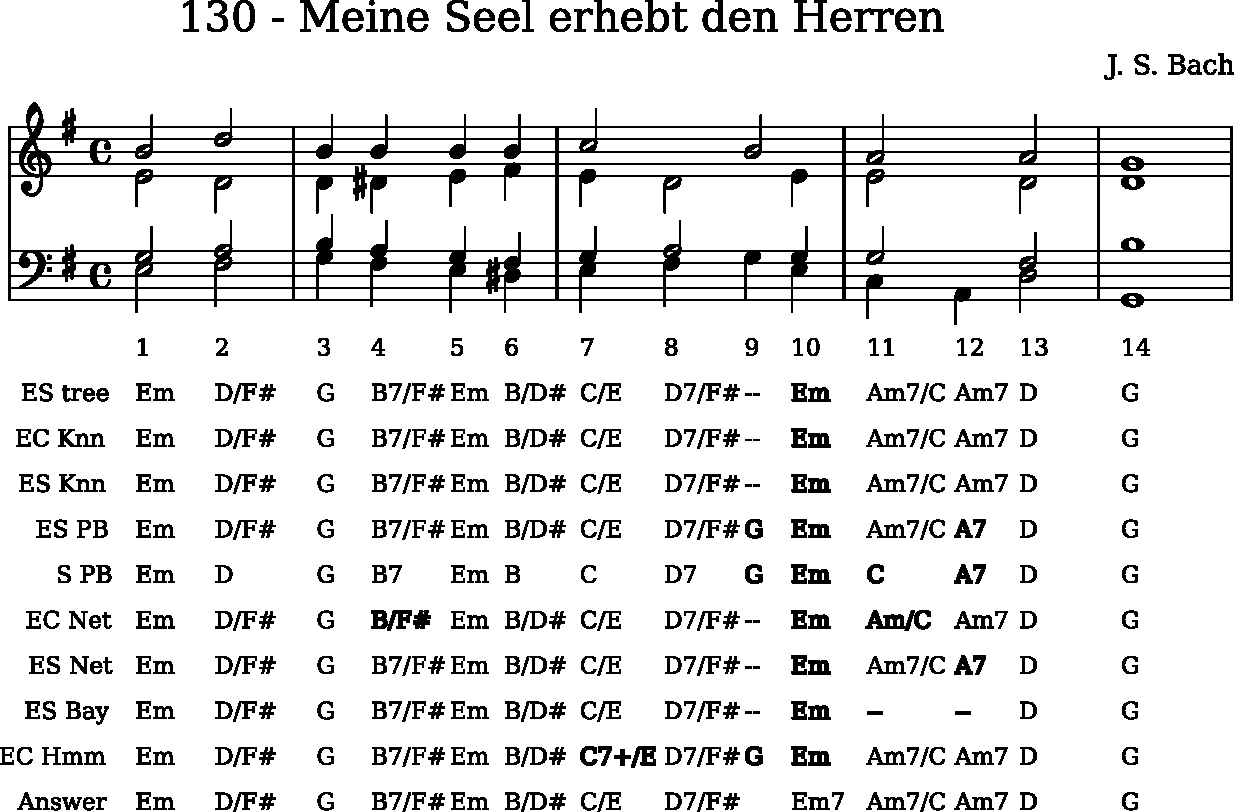
\includegraphics[scale=1.5]{analysis-130}
  \caption{Chord name analysis}
  \label{fig:chord-name-analysis}
\end{figure}
\begin{figure}
  \centering
  \includegraphics[scale=0.4]{analysis-functional-130}  
  \caption{Roman numeral analysis}
  \label{fig:roman-analysis}
\end{figure}

\section{Algorithms}
\label{sec:algorithms}

\nota{falar sobre algoritmos (duh!)}

\nota{falar que pode retreinar coisas com opcoes na linha de comando}

\section{Computational musicology}
\label{sec:comp-music}

%% and visualization

We implemented a few musicological functions in Rameau. The goal is to
turn Rameau into a framework for computational musicology. 

There are functions to show consecutive octaves and fifths in a piece.

The function ``chords'' list the frequency of each type of chord in a
set of chorales. For instance, the type of chords in the chorale 130
is

\begin{verbatim}
 C/F#                : 4.2% (1 of 24)
 C/D#                : 4.2% (1 of 24)
 C/E                 : 4.2% (1 of 24)
 Cm7/C               : 4.2% (1 of 24)
 Cm7                 : 4.2% (1 of 24)
 C/B                 : 4.2% (1 of 24)
 Cm/C                : 4.2% (1 of 24)
 Cm/B                : 4.2% (1 of 24)
 C7                  : 4.2% (1 of 24)
 C7/F#               : 8.3% (2 of 24)
 --                  : 8.3% (2 of 24)
 Cm                  : 16.7% (4 of 24)
 C                   : 29.2% (7 of 24)
\end{verbatim}

Not surprisingly, the simple major and minor triad account for the
majority of chord types. But 8.3\% are non-chords (marked with a
double dash).

Rameau can also find passages where there are voice crossings, find
range of voices and compare with textbook definition, melodic jumps
(to analyze vocal writing) and how the seventh of chords are resolved.

    Collect stats on how many chord
progressions found in the chorales are strong, weak, superstrong and
neutral, according to Schoenberg's theory of harmony.

  Voice crossing (57\% of Bach Chorales)

Consecutive octaves (4\%)

\begin{figure}[!h]
  \centering
  \subfloat[Chorale 35]{
    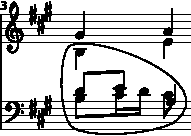
\includegraphics[scale=3]{035-16-20-cruzamento}
    \label{fig:035-cruzamento}
  }
  \subfloat[Chorale 290]{
    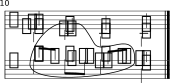
\includegraphics[scale=3]{290-66-74-cruzamento}
    \label{fig:290-66-74-cruzamento}
  } \\
  \subfloat[Chorale 3]{
    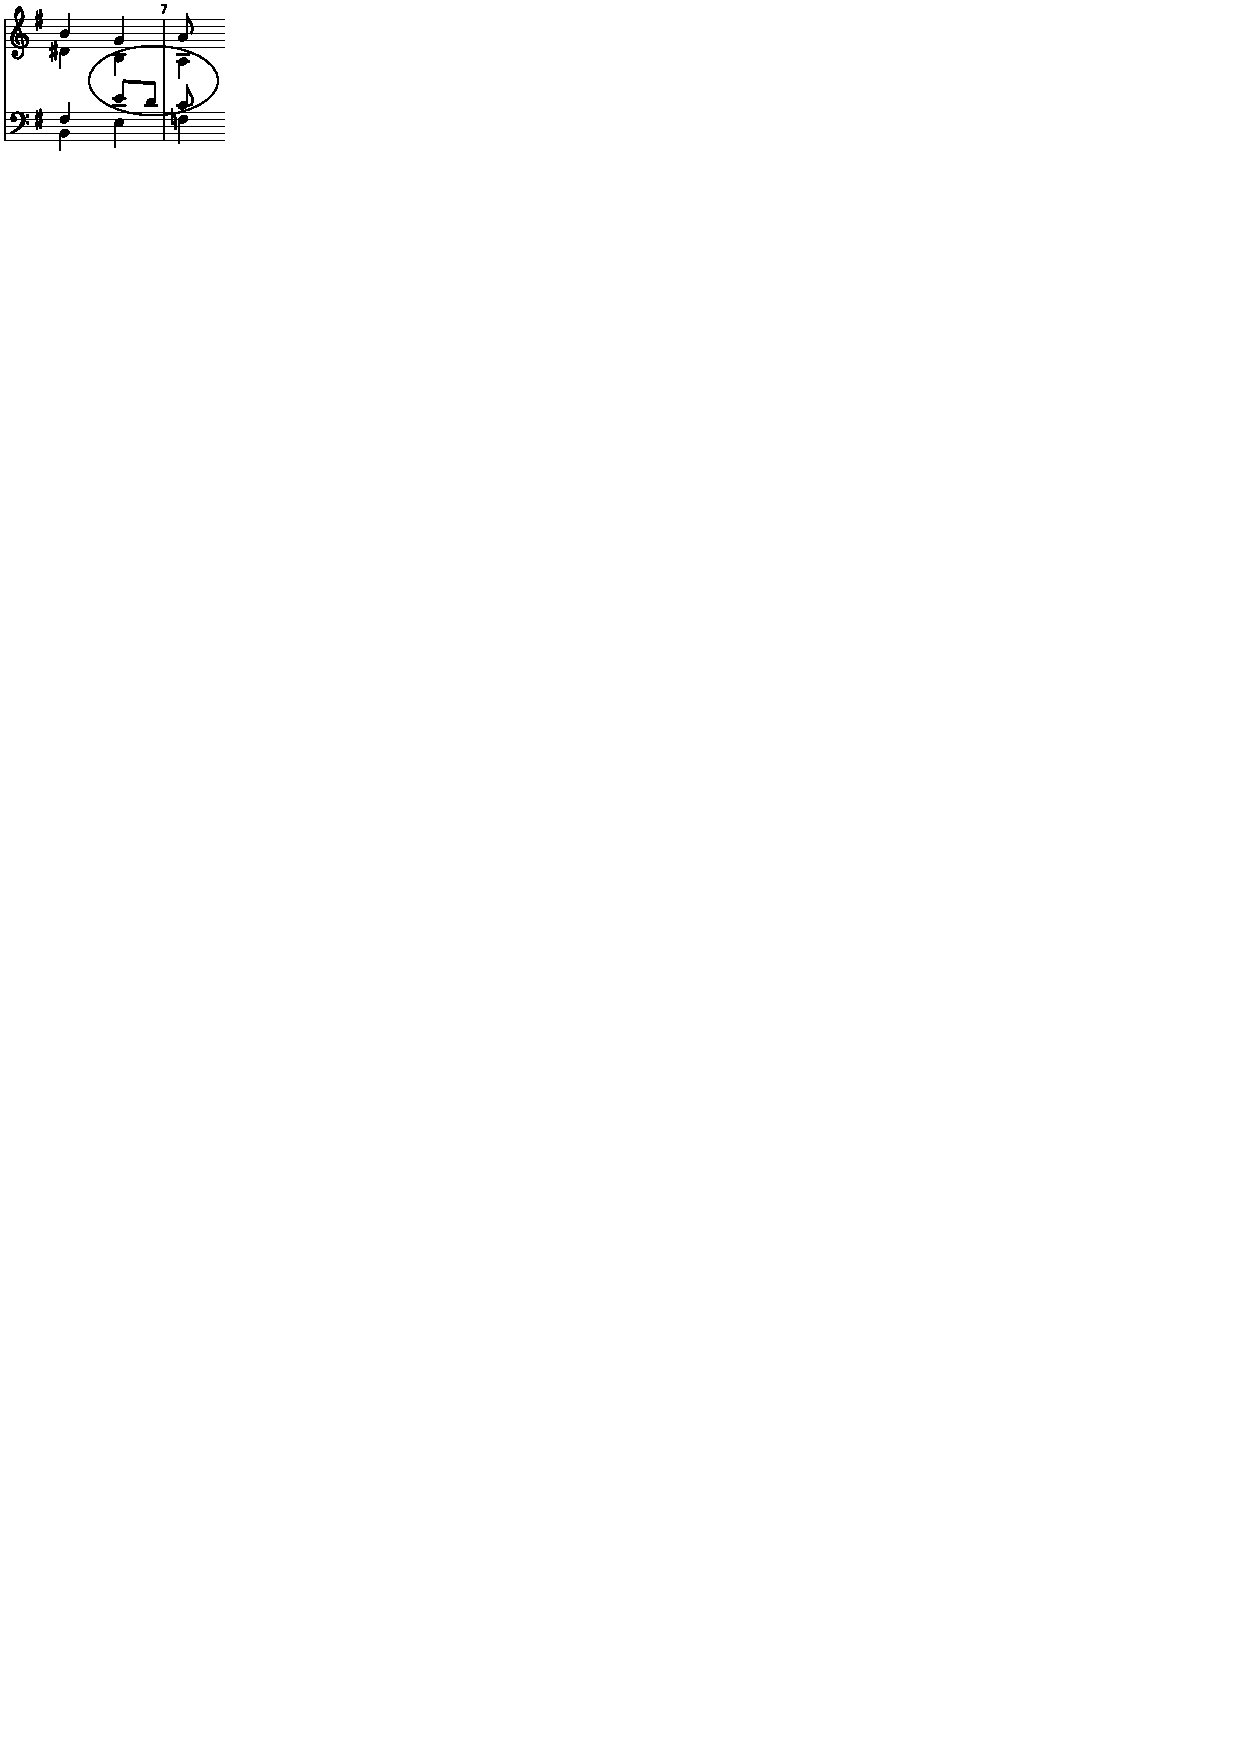
\includegraphics[scale=3]{003-38-42-cruzamento}
    \label{fig:003-38-42-cruzamento}
  }
  \caption{Cruzamentos entre vozes}
  \label{fig:coral-003}
\end{figure}

Finally, rameau can analyze the final cadence of the chorales and show

    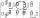
\includegraphics[scale=6]{244-oitava}
    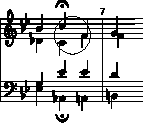
\includegraphics[scale=3]{279-oitava}
    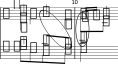
\includegraphics[scale=3]{329-oitava}

  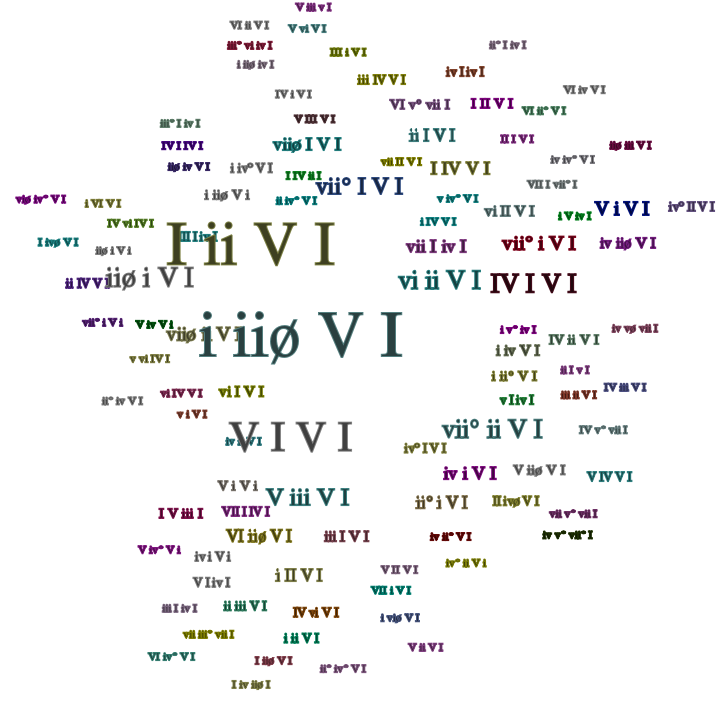
\includegraphics[scale=0.3]{cadences}

\section{Conclusion}
\label{sec:conclusion}


%%% Local Variables: 
%%% mode: latex
%%% TeX-master: "icmc2009"
%%% End: 
